\documentclass[../main]{subfiles}

\begin{document}
\chapter{Evaluation}
\label{ch:evaluation}
This chapter details a comprehensive evaluation of breast cancer classification models, implemented using transfer learning-based architectures, and includes Grad-CAM visualisations for explainability. The objective of this is to critically determine the performance of the models across several metrics such as quantitative accuracy on the test data, robustness, and generalisability to unseen data, as well as interpretability through explainable AI. A reflection on the strengths, and weaknesses of the prototype is also provided, along with a discussion on the potential for future work. The evaluation was guided by a combination of empirical metrics, and a quantitative analysis.

\section{Evaluation Methodology}
\label{sec:evaluation-methodology}
The evaluation methodology employed in this project seeks to answer the following research questions.
\begin{itemize}
    \item How accurately do models classify mammogram images?
    \item How robust and generalisable are the models to unseen data?
    \item How interpretable are the model predictions, and what insights can be derived from Grad-CAM visualisations?
    \item What potential improvements can be made for future work?
\end{itemize}

To answer these questions, the evaluation process involved the following:
\begin{itemize}
    \item \textbf{Quantitative Analysis} \textemdash\ Assessing the performance of the models using metrics such as accuracy, precision, recall, and F1 score on the test data set.
    \item \textbf{Robustness and Generalisability} \textemdash\ Evaluating the performance of the models on unseen data to determine its robustness and generalisability.
    \item \textbf{Explainable AI} \textemdash\ Using Grad-CAM visualisations to interpret the predictions of the models, and gain insight into the decision-making process.
    \item \textbf{Reflection} \textemdash\ Critically reflecting on the strengths and weaknesses of the project, and discussing potential improvements for future work.
\end{itemize}

\section{Quantitative Results}
\label{sec:quantitative-results}
The models were evaluated on a test data set of mammogram images, which is distinct from the training data set to measure generalisability more effectively. As discussed previously, the evaluation metrics used include accuracy, precision, recall, and F1 score, as well as AUC score.

\subsection{Custom CNN-based Model}
The first model, a Convolutional Neural Network (CNN) with the same classifier head as the other models, but a customised base architecture, yielded solid results. According to Table \ref{tab:quantitative-results-custom-cnn}, the model achieved an overall accuracy of 0.88, indicating that 88\% of the predictions were correct. The precision, and recall scores for the negative class were 0.96, and 0.89, respectively, indicating a strong ability to identify negative cases, while the positive class had lower scores of 0.52 for precision, and 0.74 for recall, suggesting that the model struggled to identify positive cases effectively. The F1 score averaged at 0.77 across both classes, reflecting a balance between precision, and recall. The macro average scores of 0.74 for precision, and 0.82 for recall indicate a moderate performance across both classes, while the weighted averages of 0.90 for precision, and 0.88 for recall reflect the model's overall effectiveness.

\begin{table}[h!]
    \centering
    \begin{tabular}{|l|c|c|c|c|}
        \hline
         & Precision & Recall & F1 score & Support \\ \hline
        Negative & 0.96 & 0.89 & 0.93 & 13360.00 \\ \hline
        Positive & 0.52 & 0.74 & 0.61 & 2004.00 \\ \hline
        Accuracy & 0.88 & 0.88 & 0.88 & 0.88 \\ \hline
        Macro Avg. & 0.74 & 0.82 & 0.77 & 15364.00 \\ \hline
        Weighted Avg. & 0.90 & 0.88 & 0.88 & 15364.00 \\ \hline
    \end{tabular}
    \caption{Quantitative results of the custom CNN model.}
    \label{tab:quantitative-results-custom-cnn}
\end{table}

\noindent The confusion matrix shown in Table \ref{tab:confusion-matrix-custom-cnn} reveals that of the actual negative cases, 11,955 were correctly predicted as negative, while 1,405 were incorrectly predicted as positive. This indicates a low false positive rate. However, for actual positive cases, 512 were correctly classified as positive, while 1,492 were mistakenly classified as negative, showing a high false negative rate. This suggests that the model has a strong ability to identify negative cases, but struggles with positive cases.

\begin{table}[h!]
    \centering
    \begin{tabular}{|c|c|c|}
        \hline
        \multirow{2}{*}{Actual} & \multicolumn{2}{c|}{Predicted} \\ \cline{2-3}
                                & Negative         & Positive         \\ \hline
        Negative                & 11955            & 1405              \\ \hline
        Positive                & 512              & 1492              \\ \hline
    \end{tabular}
    \caption{Confusion matrix results of the custom CNN model.}
    \label{tab:confusion-matrix-custom-cnn}
\end{table}

\noindent The Receiver Operating Characteristic (ROC) curve in Figure \ref{fig:roc-custom-cnn} for this model shows a moderate upward trend from a low false positive rate to a high true positive rate, indicating a reasonable ability to discriminate between positive, and negative classes. The area under the ROC curve (AUC) is 0.88, which indicates a good ability to distinguish between the two classes but with room for improvement.

\begin{figure}[h!]
	\centering
	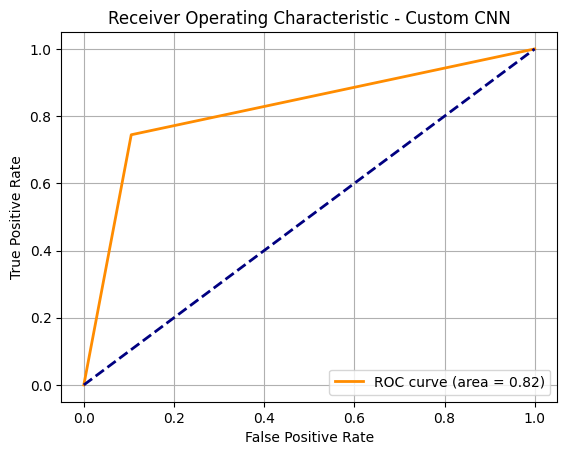
\includegraphics[width=0.8\textwidth]{assets/roc_custom_cnn.png}
	\caption{ROC curve for the custom CNN model.}
    \label{fig:roc-custom-cnn}
\end{figure}

\clearpage

\subsection{VGG16-based Model}
The VGG16-based model yielded the following results. These results, detailed in Table \ref{tab:quantitative-results-vgg16}, demonstrate robust performance with an overall accuracy of 0.96, indicating a 96\% success rate in predicting actual outcomes. As for precision, and recall scores, both averaged 0.91, and 0.92 at the macro level, demonstrating a strong balance in identifying positive, and negative cases, with precision reflecting a 91\% likelihood that positive predicitons are valid, and recall showing that 92\% of actual positives were correctly categorised. The F1 score, also averaging 0.92, denotes the effectiveness of the model by harmonising precision, and recall, highlighting its reliability over both classes. These metrics altogether imply that the model is well-performing, although minuscule variations like higher precision, and recall scores for the negative class compared to those of the positive class indicate potential areas for improvement in handling the positive class more effectively.

\begin{table}[h!]
    \centering
    \begin{tabular}{|l|c|c|c|c|}
        \hline
         & Precision & Recall & F1 score & Support \\ \hline
        Negative & 0.98 & 0.96 & 0.97 & 13360.00 \\ \hline
        Positive & 0.76 & 0.90 & 0.83 & 2004.00 \\ \hline
        Accuracy & 0.95 & 0.95 & 0.95 & 0.95 \\ \hline
        Macro Avg. & 0.87 & 0.93 & 0.90 & 15364.00 \\ \hline
        Weighted Avg. & 0.96 & 0.95 & 0.95 & 15364.00 \\ \hline
    \end{tabular}
    \caption{Quantitative results of the VGG16-based model.}
    \label{tab:quantitative-results-vgg16}
\end{table}

\noindent The confusion matrix, detailed in Table \ref{tab:confusion-matrix-vgg16}, reveals the performance of the classification model, where of the actual negative cases, 13,055 were correctly predicted negative, while 305 were incorrectly predicted positive. This indicates a low false positive rate. On the other hand, for actual positive cases, 1,718 cases were correctly labelled as positive, while 286 were mistakenly classified as negative, showing a moderate false negative rate. The model shows a strong accuracy in identifying negative cases, with a high true negative rate. This may be due to the relatively larger number of negative cases within the training data set. Overall, the confusion matrix indicates a reliable model, with further enhancements to be made to enhance sensitivity to positive cases.

\begin{table}[h!]
    \centering
    \begin{tabular}{|c|c|c|}
        \hline
        \multirow{2}{*}{Actual} & \multicolumn{2}{c|}{Predicted} \\ \cline{2-3}
                                & Negative         & Positive         \\ \hline
        Negative                & 12805            & 555              \\ \hline
        Positive                & 198              & 1806              \\ \hline
    \end{tabular}
    \caption{Confusion matrix results of the VGG16-based model.}
    \label{tab:confusion-matrix-vgg16}
\end{table}

\noindent The Receiver Operating Characteristic (ROC) curve for this model, shown in \ref{fig:roc-vgg16}, shows a significant upward trend from a low false positive rate to a high true positive rate, showing a strong discrimination ability. The area under the ROC curve, also known as AUC, is excellent at 0.92, denoting a strong ability to distinguish between positive, and negative classes. Overall, the curve indicates that the model effectively balances between sensitivity, and specificity, implying that the model is reliable for classifying benign from malignant tissue.

\begin{figure}[h!]
	\centering
	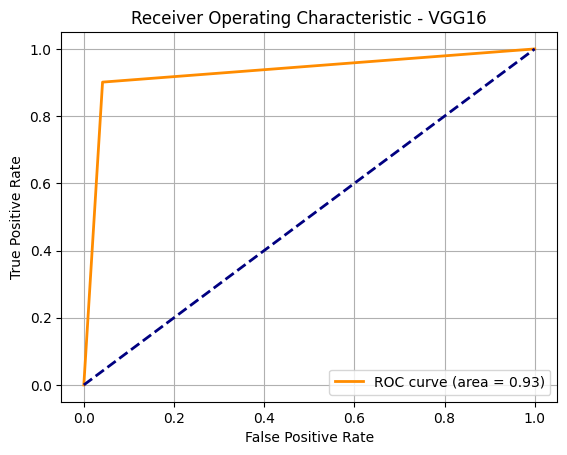
\includegraphics[width=0.8\textwidth]{assets/roc_vgg16.png}
	\caption{ROC curve for the VGG16 model.}
    \label{fig:roc-vgg16}
\end{figure}

\clearpage

\subsection{ResNet50-based Model}
The classification results for the ResNet-based model, detailed in Table \ref{tab:quantitative-results-resnet}, indicate a highly effective performance, with an overall accuracy of 0.97, implying that 97\% of predictions are correct. Both precision, and recall scores for the negative class are robust at 0.98, meaning excellent identification of negative instances supported by a large sample size of 13.360. For the positive class, precision, and recall are slightly lower at 0.90, and 0.89 but are still strong, with a support of 2,004, showing consistent performance across both classes. The macro average of 0.94 for precision, recall, and F1 score demonstrates a balanced model performance, while the weighted average of 0.97 aligns with the overall accuracy of the model, accounting for class imbalance. These results together demonstrate a reliable model with some improvements to be made in positive class predictions.

\begin{table}[h!]
    \centering
    \begin{tabular}{|l|c|c|c|c|}
        \hline
         & Precision & Recall & F1 score & Support \\ \hline
        Negative & 0.99 & 0.98 & 0.98 & 13360.00 \\ \hline
        Positive & 0.85 & 0.91 & 0.88 & 2004.00 \\ \hline
        accuracy & 0.97 & 0.97 & 0.97 & 0.97 \\ \hline
        Macro Avg. & 0.92 & 0.94 & 0.93 & 15364.00 \\ \hline
        Weighted Avg. & 0.97 & 0.97 & 0.97 & 15364.00 \\ \hline
    \end{tabular}
    \caption{Quantitative results of the ResNet50-based model.}
    \label{tab:quantitative-results-resnet}
\end{table}

\noindent The results of the confusion matrix, in Table \ref{tab:confusion-matrix-resnet}, demonstrate that 13,158 images were correctly predicted as negative, only 202 incorrectly labelled as positive, reflecting a very low false positive rate. In terms of actual positive cases, 1,777 were correctly classified as positive, while 227 were labelled incorrectly as negative, showing a moderate false negative rate. This shows a highly performing model with good precision in negative predictions.

\begin{table}[h!]
    \centering
    \begin{tabular}{|c|c|c|}
        \hline
        \multirow{2}{*}{Actual} & \multicolumn{2}{c|}{Predicted} \\ \cline{2-3}
                                & Negative         & Positive         \\ \hline
        Negative                & 13040            & 320              \\ \hline
        Positive                & 182              & 1822              \\ \hline
    \end{tabular}
    \caption{Confusion matrix results of the ResNet50-based model.}
    \label{tab:confusion-matrix-resnet}
\end{table}

\noindent The ROC curve for this model, shown in Figure \ref{fig:roc-resnet}, indicates a sharp rise from a low FPR to a high TPR, which shows a robust ability to discriminate. With an AUC score of 0.94, this model exhibits an excellent capability to distinguish between positive, and negative classes, reflecting a high balance of sensitivity, and specificity.

\begin{figure}[h!]
	\centering
	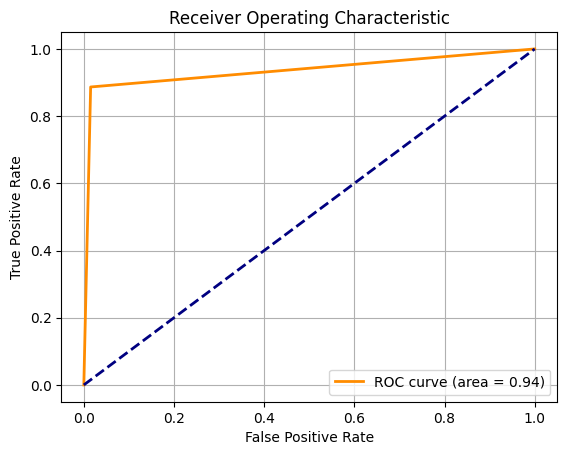
\includegraphics[width=0.8\textwidth]{assets/roc_resnet.png}
	\caption{ROC curve for the ResNet model.}
    \label{fig:roc-resnet}
\end{figure}

\clearpage

\subsection{Vision Transformer Model}
The Vision Transformer (ViT) model, which is a more recent architecture, also yielded strong results. According to Table \ref{tab:quantitative-results-vit}, the model achieved an overall accuracy of 0.97, indicating a high level of performance in classifying mammogram images. The precision, recall, and F1 score for the negative class were 0.98, 0.99, and 0.98, respectively, demonstrating excellent performance in identifying negative cases. For the positive class, precision was 0.92, recall was 0.87, and F1 score was 0.89, indicating solid performance but with room for improvement in identifying positive cases. The macro average scores of 0.95 for precision and 0.93 for recall indicate a balanced performance across both classes, while the weighted averages of 0.97 for all metrics reflect the model's overall effectiveness.

\begin{table}[h!]
    \centering
    \begin{tabular}{|l|c|c|c|c|}
        \hline
         & Precision & Recall & F1 score & Support \\ \hline
        Negative & 0.98 & 0.99 & 0.98 & 13360.00 \\ \hline
        Positive & 0.92 & 0.87 & 0.89 & 2004.00 \\ \hline
        accuracy & 0.97 & 0.97 & 0.97 & 0.97 \\ \hline
        Macro Avg. & 0.95 & 0.93 & 0.94 & 15364.00 \\ \hline
        Weighted Avg. & 0.97 & 0.97 & 0.97 & 15364.00 \\ \hline
    \end{tabular}
    \caption{Quantitative results of the ViT-based model.}
    \label{tab:quantitative-results-vit}
\end{table}

\noindent Accordinf to Table \ref{tab:confusion-matrix-vit}, the confusion matrix for the ViT model shows that 13,214 images were correctly predicted as negative, with only 146 incorrectly labelled as positive, indicating a very low false positive rate. For the actual positive cases, 1,737 were correctly classified as positive, while 267 were incorrectly labelled as negative, showing a moderate false negative rate. This indicates that the model performs well in identifying negative cases, but there is still room for improvement in identifying positive cases.

\begin{table}[h!]
    \centering
    \begin{tabular}{|c|c|c|}
        \hline
        \multirow{2}{*}{Actual} & \multicolumn{2}{c|}{Predicted} \\ \cline{2-3}
                                & Negative         & Positive         \\ \hline
        Negative                & 13214            & 146              \\ \hline
        Positive                & 267              & 1737              \\ \hline
    \end{tabular}
    \caption{Confusion matrix results of the ViT-based model.}
    \label{tab:confusion-matrix-vit}
\end{table}

\noindent The ROC curve for the ViT model, shown in \ref{fig:roc-vit}, shows a strong upward trend from a low false positive rate to a high true positive rate, indicating a robust ability to discriminate between positive, and negative classes. The AUC score of 0.93 reflects an excellent ability to distinguish between the two classes, demonstrating a high balance of sensitivity, and specificity.

\begin{figure}[h!]
	\centering
	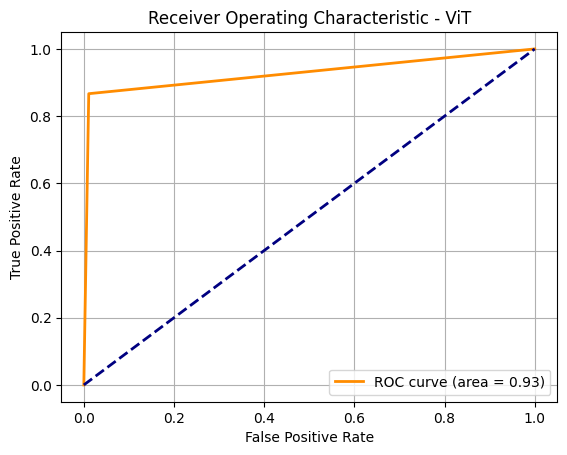
\includegraphics[width=0.8\textwidth]{assets/roc_vit.png}
	\caption{ROC curve for the ViT model.}
    \label{fig:roc-vit}
\end{figure}

\clearpage

\section{Comparing the Models}
\label{sec:comparing-models}
The custom CNN network is considered as a baseline. The quantitative results of the four models indicate that all models perform well, with the ResNet50-based model achieving the highest accuracy of 0.97, with almost identical results to the ViT model, closely followed by the VGG16-based model at 0.96, and the custom CNN-based model at 0.88. The precision, recall, and F1 score metrics also reflect strong performance across all models, with the ResNet50-based model showing the best balance between precision, and recall for both classes. The graph \ref{fig:comparison-models} demonstrates the comparison of the models between training epochs in terms of accuracy, and loss scores.

\begin{figure}[h!]
    \centering
    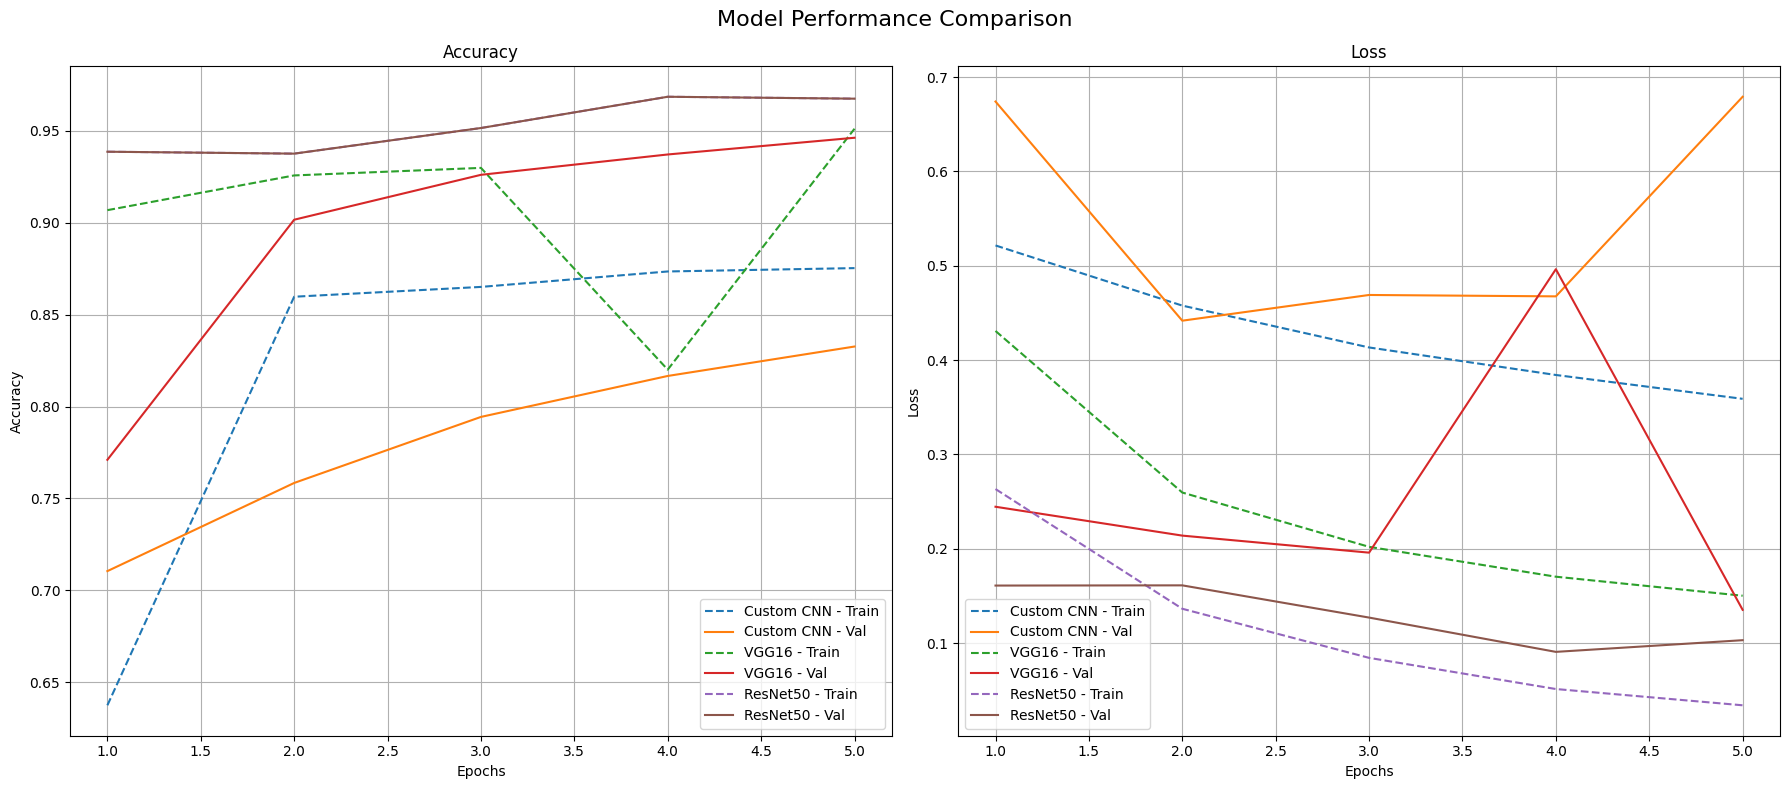
\includegraphics[width=1\textwidth]{assets/comparison.png}
    \caption{Comparison of the CNN models across training epochs in terms of accuracy, and loss scores.}
    \label{fig:comparison-models}
\end{figure}

\noindent The ROC curves for all models show a strong ability to discriminate between positive, and negative classes, with AUC scores ranging from 0.88 to 0.94, indicating a high balance of sensitivity, and specificity. The confusion matrices further highlight the strengths, and weaknesses of each model, with the ResNet50-based model showing the best performance in terms of true positive, and true negative rates.

\section{Explainablity}
\label{sec:explainability}
In order to assess the model's performance on predictions aligned with human-interpretable features, a series of images is presented with Grad-CAM overlays. This analysis can be implemented in a clinical system, which would allow radiologists to interpret, and trust decisions made by a CNN-based system. The ability to visually validate the reasoning process behind each decision increases trust in the system, and reduces the opacity of models, and aids in the diagnosis of errors.

Overall, the use of Grad-CAM significantly improves the usability of the models in real-world situations, enabling the effective collaboration between human radiologists, and machines. Namely, in future studies, radiologists could rate the consistency, and usefulness of heatmaps on a Likert scale or utilise them to flag low-confidence cases for further review. Below are some of the images with Grad-CAM overlays, demonstrating the model's focus on relevant features in the mammogram images.

\begin{figure}[h!]
    \centering
    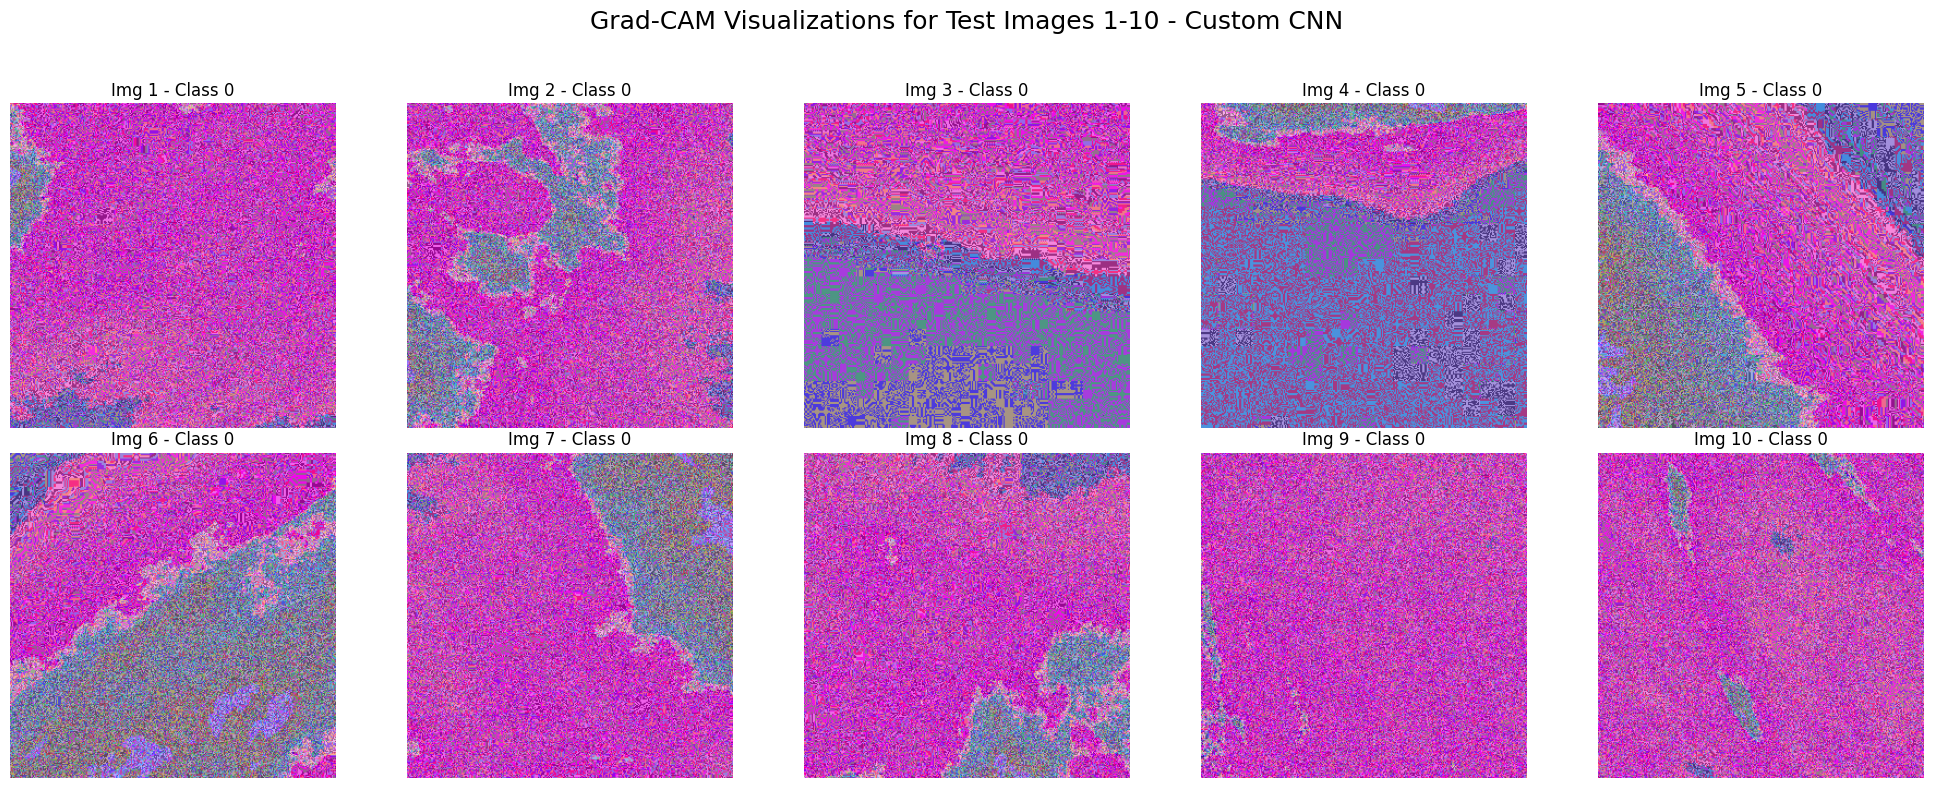
\includegraphics[width=0.8\textwidth]{assets/grad_cam_custom_cnn.png}
    \caption{Example of Grad-CAM overlay on a mammogram image for the custom CNN.}
    \label{fig:grad-cam-custom-cnn}
\end{figure}

\begin{figure}[h!]
    \centering
    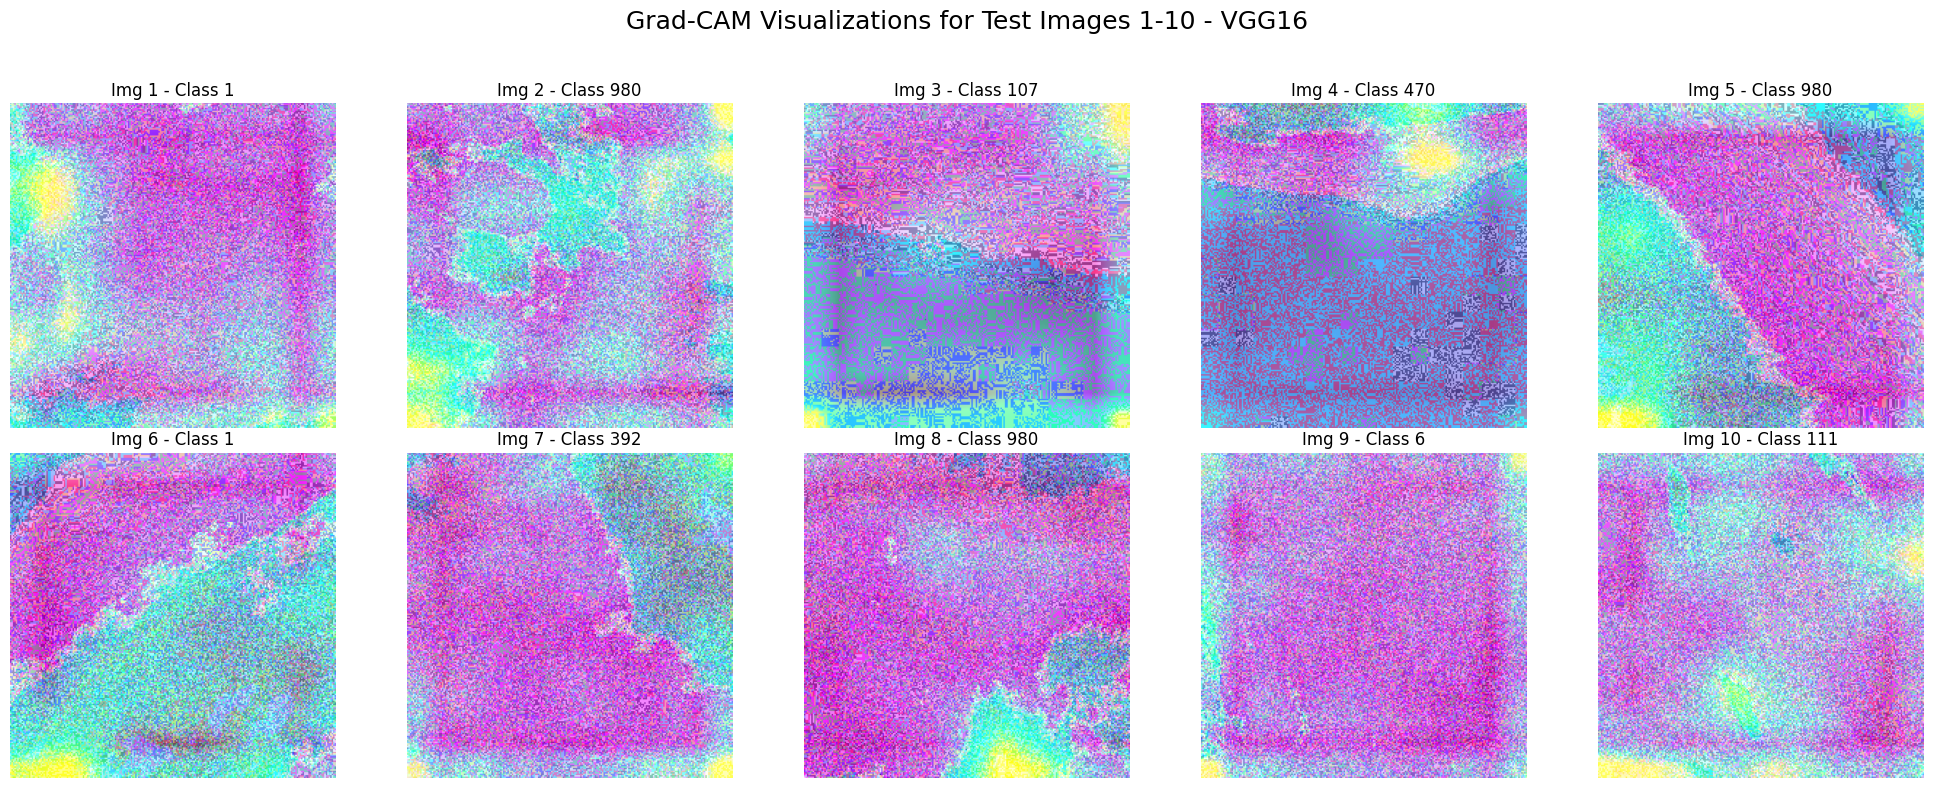
\includegraphics[width=0.8\textwidth]{assets/grad_cam_vgg16.png}
    \caption{Example of Grad-CAM overlay on a mammogram image for the VGG16-based network.}
    \label{fig:grad-cam-vgg16}
\end{figure}

\begin{figure}[h!]
    \centering
    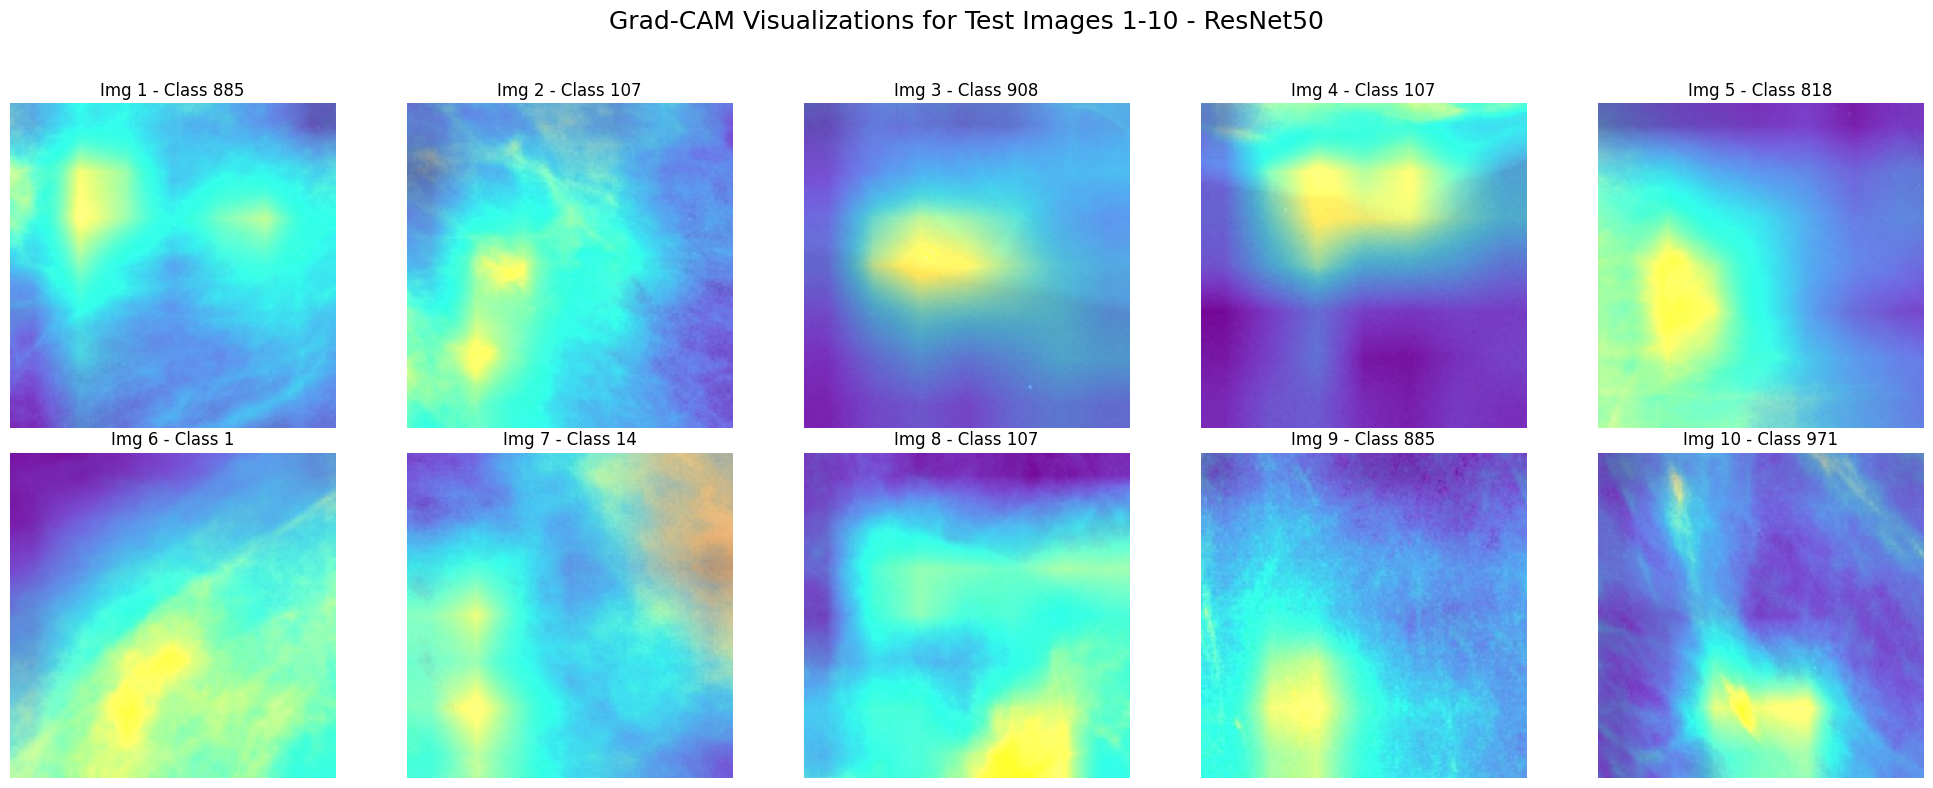
\includegraphics[width=0.8\textwidth]{assets/grad_cam_resnet50.png}
    \caption{Example of Grad-CAM overlay on a mammogram image for the ResNet50-based network.}
    \label{fig:grad-cam-resnet50}
\end{figure}

\begin{figure}[h!]
    \centering
    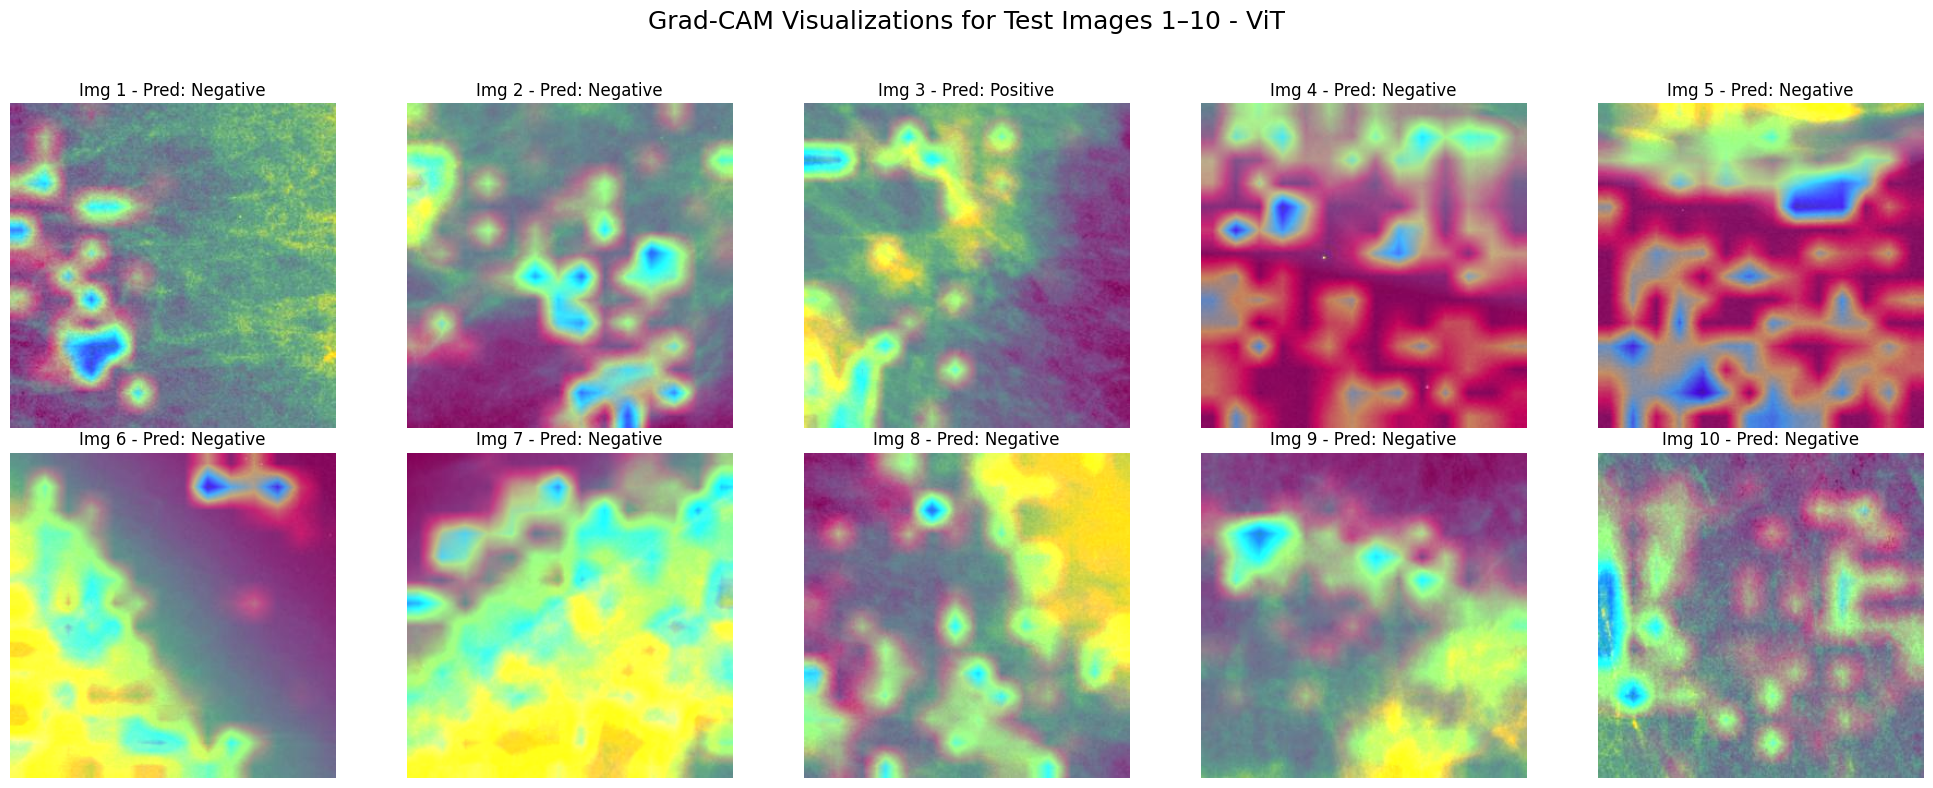
\includegraphics[width=0.8\textwidth]{assets/grad_cam_vit.png}
    \caption{Example of Grad-CAM overlay on a mammogram image for the ViT-based network.}
    \label{fig:grad-cam-vit}
\end{figure}

\clearpage

\section{Achievements}
This project has overseen the end-to-end development of a raw TFRecord ingestion system that makes interpretable, and accurate predictions. A reasonably strong generalisation has been achieved using transfer learning on limited data, given the AUC scores. Grad-CAM has also been effectively integrated for transparency, with minimal overfitting through the use of dropout, and early stopping.

\section{Reflection}
\label{sec:reflection}
The project has successfully demonstrated the potential of deep learning-based models for breast cancer classification using mammogram images. The models have shown strong performance across various metrics, and the integration of Grad-CAM has provided valuable information on the decision-making process of the models. However, there are several areas of improvement, including:
\begin{itemize}
    \item \textbf{data set Limitations} \textemdash\ The data set used for training, and testing the models is relatively small, and imbalanced, which can limit the generalisability of the models. Although this was partially accounted for by computing, and utilising class weights, future work should focus on acquiring larger, and more diverse data sets to improve model performance.
    \item \textbf{Model Complexity} \textemdash\ While the models have shown strong performance, there is potential for further refinement, and optimisation of the architectures to improve accuracy, and reduce overfitting. Most significantly, the transformer-based model could be further optimised by increasing the number of training epochs, and using a larger transformer model with more hyperparameters.
    \item \textbf{Evaluation Methodology} \textemdash\ The evaluation methodology could be enhanced by incorporating cross-validation techniques to provide more robust metrics, and reduce the risk of overfitting.
    \item \textbf{Collaboration with Domain Experts} \textemdash\ Engaging with domain experts such as radiologists can provide valuable insights into the clinical relevance of the model predictions, and help refine the models further.
    \item \textbf{Explainability} \textemdash\ While Grad-CAM has provided valuable insights into the model predictions, further research into explainable AI techniques can enhance the interpretability of the models, and improve trust in their predictions.
\end{itemize}
These areas for improvement highlight the potential for future work, and the ongoing development of deep learning-based models for breast cancer classification.

\section{Summary}
\label{sec:summary}
This evaluation indicates that the proposed deep learning-based system performs adequately on test data, and allows for useful interpretability via Grad-CAM. While the results are promising, the system would not be ready for a production scenario due to data set constraints that could be overcome given more powerful hardware to be able to train with it. Nevertheless, a solid foundation has been laid such that further refinement, more intricate, and advanced loss functions, fine-tuning, and domain expert consultation can be made. In addition, further modifications to the evaluation of the models will be made to include cross-validation, which will give far more accurate metrics than the existing single-fold method of evaluation.

\end{document}
